\newpage
\section{Pianificazione}\label{Pianificazione}
	L'attività di pianificazione consiste nella suddivisione del lavoro tra i vari membri di \gruppo.
	Essa deve fare in modo che ogni elemento abbia la possibilità di ricoprire almeno una volta tutti i ruoli di progetto.

    Tenendo a mente le scadenze riportate alla sezione \S\ref{Scadenze}, abbiamo ritenuto opportuno dividere il lavoro in quattro macro-periodi:
	\begin{itemize}
	\item Analisi dei requisiti
	\item Progettazione della base tecnologica
	\item Progettazione di dettaglio e codifica
	\item Validazione e collaudo
	\end{itemize}

	Ogni macro-periodo è stato suddiviso in periodi più brevi (chiamati I periodo, II periodo, etc\dots) per renderne più semplice il
    controllo e la pianificazione. Per esemplificare l'intervallo di tempo tra un macro-periodo e l'altro, verranno usati vari
    diagrammi di Gantt dove sarà chiaro chi ha svolto qualsiasi attività.

    In ognuno di essi ci saranno due milestone (di colore verde):

    \begin{itemize}
    	\item Consegna dei documenti
    	\item Discussione
    \end{itemize}

    \subsection{Analisi dei requisiti}\label{PianificazioneAnalisiDeiRequisiti}
        Questo macro-periodo ha inizio il 2018-11-15. Procede con quattro periodi fino al 2019-01-14 con la consegna dei documenti e, nel
        quinto e ultimo periodo, ci prepareremo per la revisione dei requisiti del 2019-01-21.

        I ruoli attivi sono:
        \begin{itemize}
            \item Responsabile
            \item Amministratore
            \item Analista
            \item Verificatore
        \end{itemize}
        Questo macro-periodo è stata diviso in cinque periodi:
		\begin{itemize}
			\item \textbf{I periodo}: dal 2018-11-22 al 2018-12-02
			\begin{itemize}
    	        \item \textbf{Discussione capitolati}: sono stati discussi pro e contro di ogni capitolato e, dopo un periodo di
				studio e analisi, abbiamo concluso con la scelta del capitolato C1.
    	        \item \textbf{Ricerca degli strumenti}: individuazione degli strumenti di supporto da utilizzare durante il progetto.
    	        \item \textbf{Normazione}: definizione di regole per stilare i documenti.
    	        \item \textbf{Distribuzione ruoli e pianificazione attività}
       	        \item \textbf{Studio di fattibilità}
       	        \item \textbf{Pianificazione qualità}: individuazione metodi per garantire qualità del prodotto.
			\end{itemize}
			\newpage
			\item \textbf{II periodo}: dal 2018-12-03 al 2018-12-16
			\begin{itemize}
    	        \item \textbf{Normazione}: definizione di regole per i processi organizzativi.
    	        \item \textbf{Analisi dei rischi}
    	        \item \textbf{Pianificazione qualità}: individuazione dei metodi per garantire qualità del prodotto.
       	        \item \textbf{Ricerca degli strumenti}: individuazione degli strumenti per le varie attività di progetto.
       	        \item \textbf{Pianificazione attività}: diagrammi di Gantt e pianificazione dell'intero progetto.
       	        \item \textbf{Definizione \gloss{casi d'uso}}
			\end{itemize}
        	\item \textbf{III periodo}: dal 2018-12-17 al 2018-12-29
			\begin{itemize}
    	        \item \textbf{Normazione}: definizione di regole per i processi organizzativi.
    	        \item \textbf{Analisi dei requisiti}: ricerca requisiti del capitolato scelto.
       	        \item \textbf{Ricerca degli strumenti}: strumenti per interfacciarsi al \gloss{Producer} e al \gloss{Broker}.
        	\end{itemize}
        	\item \textbf{IV periodo}: dal 2018-12-30 al 2019-01-13
        	\begin{itemize}
       	        \item \textbf{Ricerca degli strumenti}: strumenti per interfacciarsi col Gestore personale e con il \gloss{Consumer}.
       	        \item \textbf{Pianificazione attività}: aggiornamenti della pianificazione.
       	        \item \textbf{Stesura lettera di presentazione}
        	\end{itemize}
        	\item \textbf{V periodo}: dal 2019-01-15 al 2019-01-20
        	\begin{itemize}
    	        \item \textbf{Preparazione per la discussione}: realizzazione della presentazione e studio personale.
        	\end{itemize}
		\end{itemize}

        \begin{landscape}
			\subsubsection{Diagramma di Gantt}
			\begin{figure}[H]
					\centering
					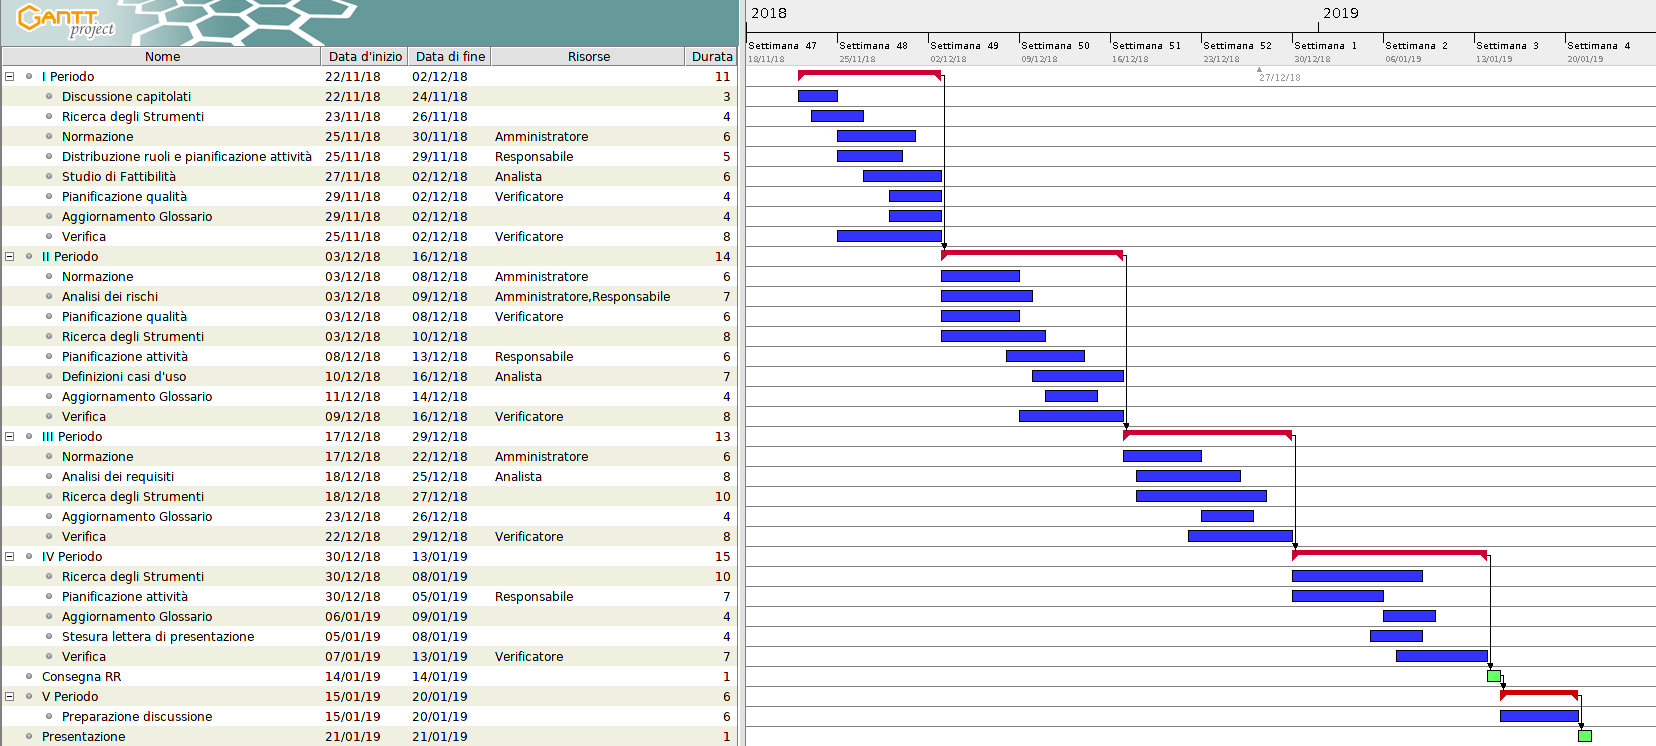
\includegraphics[scale=0.4]{img/Analisi_dei_requisiti.png}\\
					\caption{Diagramma di Gantt della macro analisi dei requisiti}
			\end{figure}
		\end{landscape}

		\newpage

        \subsection{Progettazione della base tecnologica}\label{PianificazioneBaseTecnologica}
		Questo macro-periodo ha inizio il 2019-01-22, procede con quattro periodi fino al 2019-03-15.

		In questa attività sono stati aggiunti tre rilevamenti riguardanti la qualità, a distanza di una settimana l'uno
		dall'altro. Questi ci permetteranno di avere una rappresentazione chiara del modo in cui si starà lavorando.

        I ruoli attivi sono:
        \begin{itemize}
            \item Responsabile
            \item Amministratore
            \item Analista
            \item Progettista
            \item Programmatore
            \item Verificatore
        \end{itemize}
        Questo macro-periodo è stato suddiviso in quattro periodi:
		\begin{itemize}
			\item \textbf{I periodo}: dal 2019-01-22 al 2019-02-03. È incentrato nel sistemare la struttura e i contenuti
			dei documenti a seguito della revisione e allo studio delle tecnologie utili per una corretta progettazione.
			\begin{itemize}
    	        \item \textbf{Normazione}
    	        \item \textbf{Analisi dei requisiti}: revisione in profondità di casi d'uso e requisiti.
    	        \item \textbf{Pianificazione delle attività}: aggiornamenti della pianificazione.
    	        \item \textbf{Pianificazione qualità}
    	        \item \textbf{Ricerca degli strumenti}: \gloss{GitLab}, \gloss{Redmine}, \gloss{framework} e librerie per lo sviluppo del prodotto.
        	\end{itemize}
			\item \textbf{II periodo}: dal 2019-02-04 al 2019-02-25. È il fulcro della macro-attività: viene progettato e realizzato
				il Proof of Concept. 
			\begin{itemize}
				\item \textbf{Normazione}: aggiunta nuovi strumenti utilizzati.
				\item \textbf{Progettazione}: implementazione schemi \gloss{UML}.
				\item \textbf{Ricerca degli strumenti}: \gloss{Apache Kafka}, \gloss{Docker}, \gloss{CherryPy},
				\gloss{MongoDB}, \gloss{SonarQube}.
    	        \item \textbf{Pianificazione delle attività}: aggiornamenti della pianificazione.
    	        \item \textbf{Analisi dei rischi}: aggiornamento di eventuali rischi previsti o riscontrati.
    	        \item \textbf{Codifica}: realizzazione del \gloss{Proof of Concept}.
    	        \item \textbf{Pianificazione qualità}: prima rilevazione indici per la verifica.
        	\end{itemize}
        	\item \textbf{III periodo}: dal 2019-02-27 al 2019-03-07. Viene ultimata la stesura dei documenti
				in vista della revisione di progetto del 2019-03-15. Termina il giorno prima della consegna del
				materiale in ingresso per tale revisione.
			\begin{itemize}
				\item \textbf{Pianificazione delle attività}: aggiornamenti della pianificazione.
				\item \textbf{Analisi dei requisiti}
				\item \textbf{Pianificazione qualità}: seconda rilevazione indici per la verifica.
				\item \textbf{Stesura lettera di presentazione}
				\item \textbf{Pianificazione qualità}: terza rilevazione indici per la verifica.
        	\end{itemize}
        	\item \textbf{IV periodo}: dal 2019-03-09 al 2019-03-14. Preparazione in vista della revisione.
        	\begin{itemize}
        		\item \textbf{Preparazione per la discussione}: realizzazione della presentazione e studio personale.
        	\end{itemize}
		\end{itemize}

        \begin{landscape}
			\subsubsection{Diagramma di Gantt}\label{GanttPianificazioneBaseTecnologica}
			\begin{figure}[H]
					\centering
					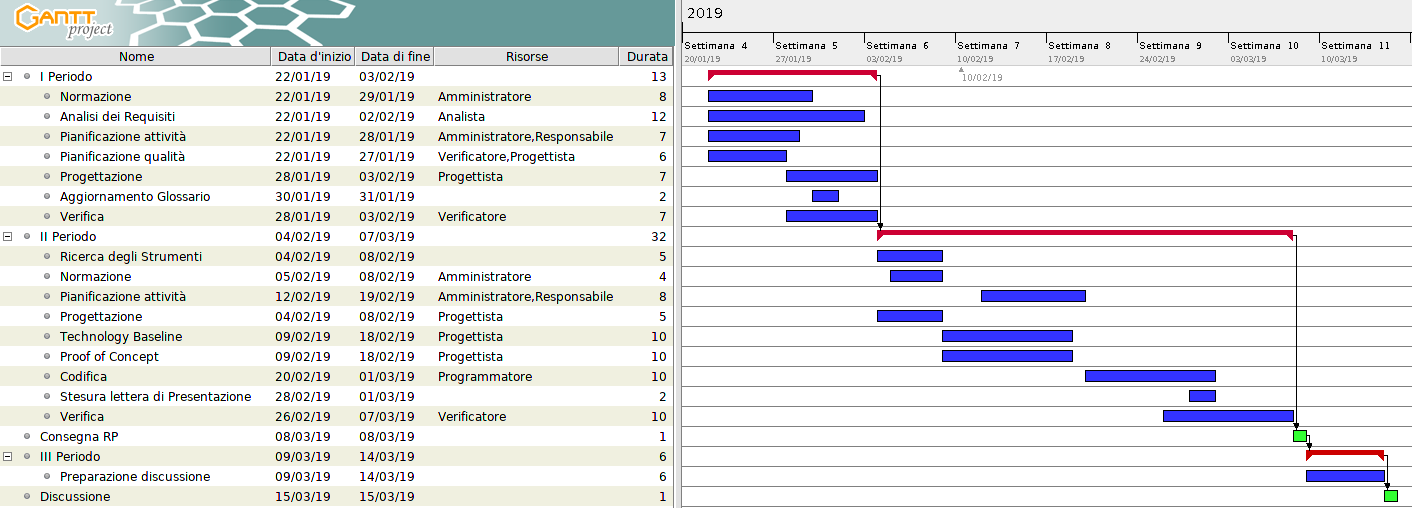
\includegraphics[scale=0.375]{img/Progettazione_della_base_tecnologica.png}\\
					\caption{Diagramma di Gantt della macro progettazione della base tecnologica}
			\end{figure}
		\end{landscape}
		\newpage

        \subsection{Progettazione di dettaglio e codifica}\label{PianificazioneDettaglio}
		Questo macro-periodo ha inizio il 2019-03-16, è diviso in quattro periodi e dura fino al 2019-04-19,
		data della revisione di qualifica.

		In questa attività sono stati aggiunti tre rilevamenti riguardanti la qualità, a distanza di una settimana l'uno
		dall'altro. Questi ci permetteranno di avere una rappresentazione chiara del modo in cui si starà lavorando.

        I ruoli attivi sono:
        \begin{itemize}
            \item Responsabile
            \item Amministratore
            \item Progettista
            \item Programmatore
            \item Verificatore
        \end{itemize}
        Questo macro-periodo è stato diviso in tre periodi:
		\begin{itemize}
			\item \textbf{I periodo}: dal 2019-03-16 al 2019-03-26. Questo periodo è incentrato nella progettazione in dettaglio
				in vista del colloquio per la Product \gloss{Baseline}, che sarà indicativamente tra il 27 e il 30 marzo 2019.
			\begin{itemize}
    	        \item \textbf{Ricerca degli strumenti}
    	        \item \textbf{Pianificazione delle attività}: aggiornamenti della pianificazione.
    	        \item \textbf{Normazione}
    	        \item \textbf{Progettazione}: miglioramento Technology Baseline e Proof of Concept.
                \item \textbf{Analisi dei requisiti}: revisione in profondità di casi d'uso e requisiti.
    	        \item \textbf{Codifica}: prima implementazione.
    	        \item \textbf{Pianificazione qualità}: prima rilevazione indici per la verifica.
        	\end{itemize}
			\item \textbf{II periodo}: dal 2019-03-27 al 2019-04-01. Questo periodo è incentrato nella realizzazione del prodotto tramite
				codifica di dettaglio ed eventuali migliorie alla progettazione.
			\begin{itemize}
				\item \textbf{Progettazione e Product Baseline}: implementazione della Product Baseline tramite diagrammi delle
				classi e di sequenza, coerentemente con quanto dichiarato nella Technology Baseline.
    	        \item \textbf{Normazione}
    	        \item \textbf{Codifica}: implementazione seguendo specifiche progettuali ed implementazione dei test.
    	        \item \textbf{Pianificazione qualità}: seconda rilevazione indici per la verifica.
    	        \item \textbf{Scrittura manuale}: prima stesura.
        	\end{itemize}
        	\item \textbf{III periodo}: dal 2019-04-03 al 2019-04-11. Come il periodo precedente, ma il focus è più incentrato nella
				scrittura dei manuali e nelle ultime attività che precedono la consegna.
			\begin{itemize}
				\item \textbf{Pianificazione attività}: aggiornamenti della pianificazione.
    	        \item \textbf{Progettazione}: scelta dei \gloss{design pattern}.
    	        \item \textbf{Codifica}: primo rilascio.
    	        \item \textbf{Pianificazione qualità}: terza rilevazione indici per la verifica.
    	        \item \textbf{Scrittura manuale}: aggiornamenti al manuale.
    	        \item \textbf{Stesura lettera di presentazione}
        	\end{itemize}
        	\item \textbf{IV periodo}: dal 2019-04-13 al 2019-04-18. Preparazione in vista della revisione.
			\begin{itemize}
				\item \textbf{Preparazione per la discussione}: realizzazione della presentazione e studio personale.
        	\end{itemize}
        \end{itemize}

        \begin{landscape}
			\subsubsection{Diagramma di Gantt}
			\begin{figure}[H]
					\centering
					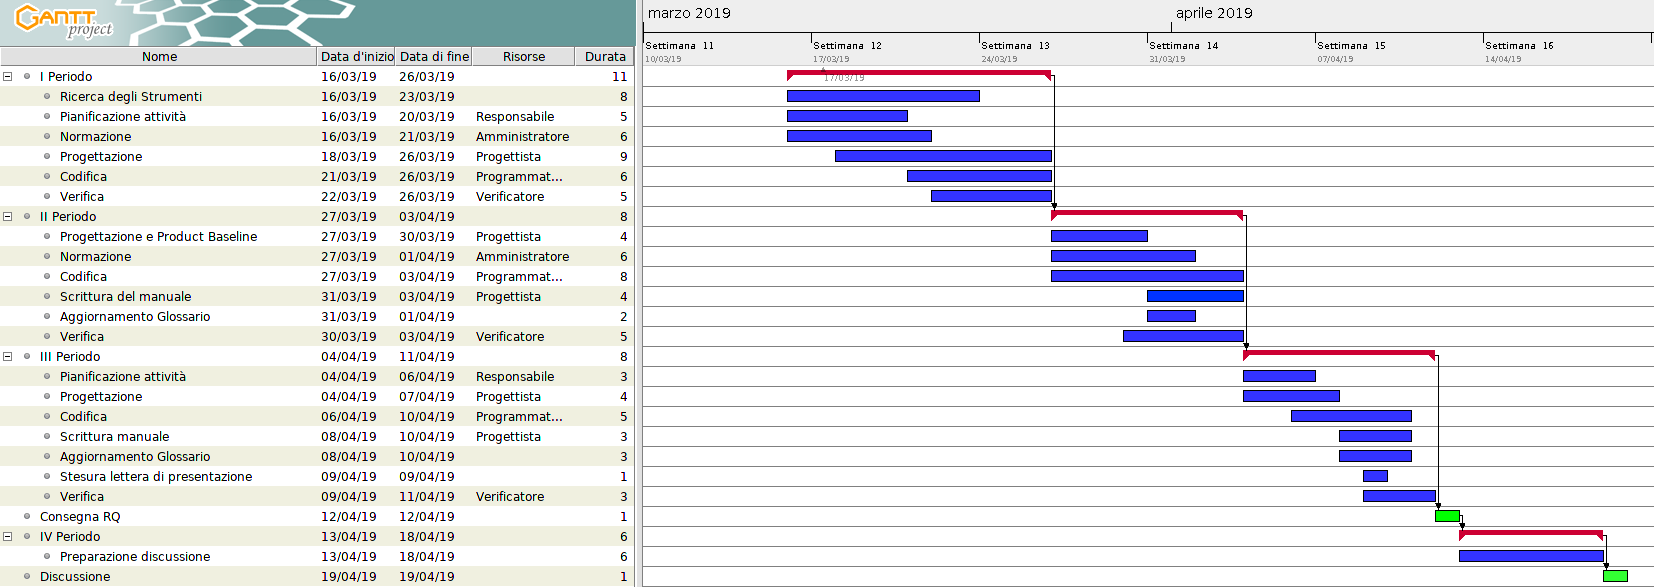
\includegraphics[scale=0.42]{img/Progettazione_di_dettaglio_e_codifica.png}\\
					\caption{Diagramma di Gantt della macro progettazione di dettaglio e codifica}
			\end{figure}
		\end{landscape}
		\newpage

        \subsection{Validazione e collaudo}\label{PianificazineValidazione}
		Questo macro-periodo ha inizio il 2019-04-20, procede con tre periodi e la vigilia della Revisione di Accettazione va consegnato il materiale in
        ingresso. La Revisione è prevista per il 2019-05-17.

        I ruoli attivi sono:
        \begin{itemize}
            \item Amministratore
            \item Responsabile
            \item Verificatore
		\end{itemize}

        Questo macro-periodo è stato diviso in tre periodi:
		\begin{itemize}
			\item \textbf{I periodo}: dal 2019-04-20 al 2019-04-30
			\begin{itemize}
    	        \item \textbf{Normazione}
    	        \item \textbf{Pianificazione attività}: aggiornamenti pianificazione.
                \item \textbf{Scrittura dei manuali}: completamento manuali.
    	        \item \textbf{Pianificazione qualità}:  prima rilevazione indici per la verifica.
    	        \item \textbf{Raffinamento specifiche}: completamento delle specifiche.
        	\end{itemize}
			\item \textbf{II periodo}: dal 2019-05-01 al 2019-05-09
			\begin{itemize}
    	        \item \textbf{Codifica}: completamento ultima versione.
                \item \textbf{Pianificazione qualità}:  seconda rilevazione indici per la verifica.
    	        \item \textbf{Scrittura dei manuali}: completamento manuali.
                \item \textbf{Pianificazione qualità}:  terza rilevazione indici per la verifica.
    	        \item \textbf{Test e collaudo}: esecuzione di test di collaudo e ultimi miglioramenti del prodotto per
    	        garantire che questo soddisfi tutti i vincoli qualitativi.
			\end{itemize}
			\item \textbf{III periodo}: dal 2019-05-10 al 2019-05-15
			\begin{itemize}
				\item \textbf{Preparazione discussione}: realizzazione della presentazione, studio personale e preparazione demo per il collaudo.
			\end{itemize}
		\end{itemize}

        \begin{landscape}
			\subsubsection{Diagramma di Gantt}
			\begin{figure}[H]
					\centering
					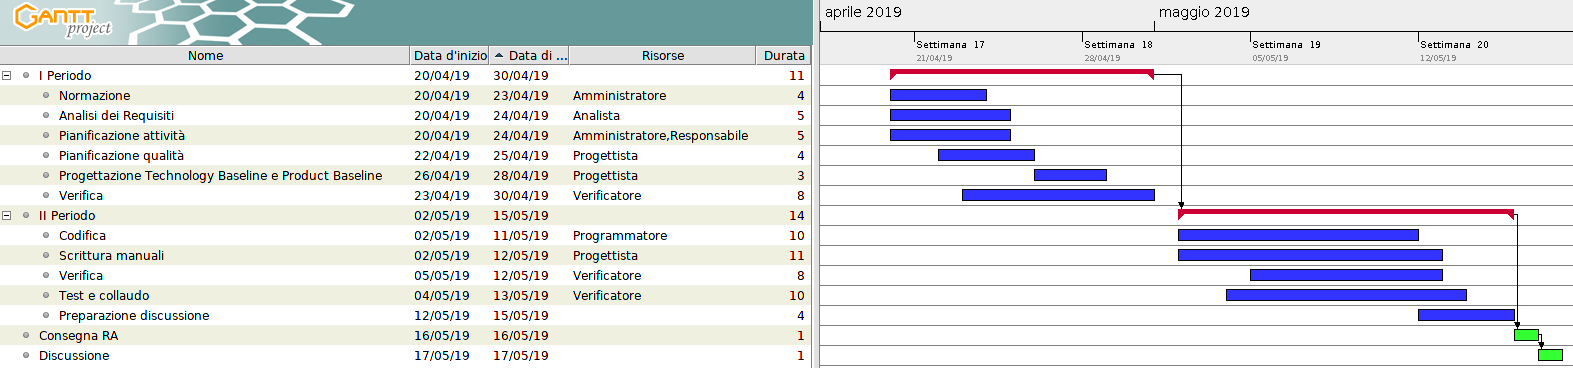
\includegraphics[scale=0.43]{img/Validazione_e_collaudo.png}\\
					\caption{Diagramma di Gantt della macro validazione e collaudo}
			\end{figure}
		\end{landscape}
		\newpage
